\documentclass[12pt]{article}

\usepackage[margin=0.5in]{geometry}

\usepackage{hyperref}
\hypersetup{
    colorlinks=true,
    linkcolor=blue,
    filecolor=magenta,      
    urlcolor=blue,
}
 
\urlstyle{same}

\usepackage{datetime}
\newdateformat{specialdate}{\twodigit{\THEDAY}.\twodigit{\THEMONTH}.\THEYEAR}

\usepackage{polski}
\usepackage[polish]{babel}
\usepackage[utf8]{inputenc}

\usepackage{titling}

\usepackage{framed}
\usepackage[svgnames]{xcolor}
\colorlet{shadecolor}{Gainsboro!50}

\usepackage{float}
\usepackage{graphicx}
\graphicspath{ {./images/} }

\usepackage{verbatim}

\usepackage{caption}
\captionsetup[figure]{name=Fig.}

\title{Consensus trees}
\author{Maciej Sikora}
\date{\specialdate\today}


\begin{document}
\maketitle

Uliniowienie wykonane z pomocą pakietu mafft.

Drzewa Neighbor Joining wykonane zostały z użyciem pakietu PhyML.

Drzewa konsensusowe  wyliczone zostały z użyciem pakietu Bio.Phylo.

Wyniki dla metody strict przewidywalnie nie były najlepsze:
\begin{figure}[H]
\begin{center}
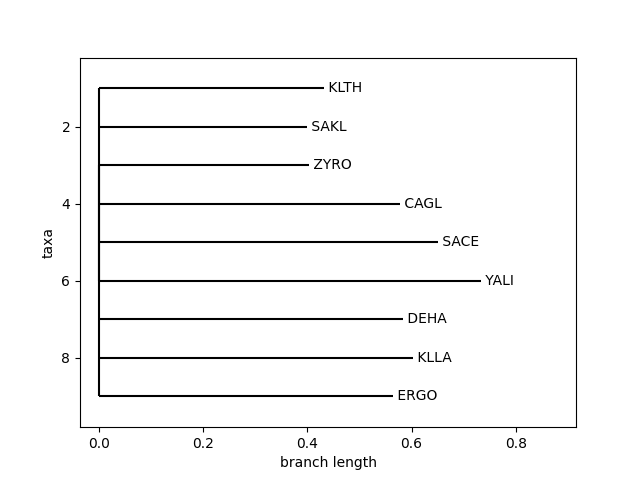
\includegraphics[width=0.7\textwidth]{strict}
\end{center}
\end{figure}


Dla metody majority z wartością cutoff = 0.3 uzyskane zostało jednak następujące drzewo.
\begin{figure}[H]
\begin{center}
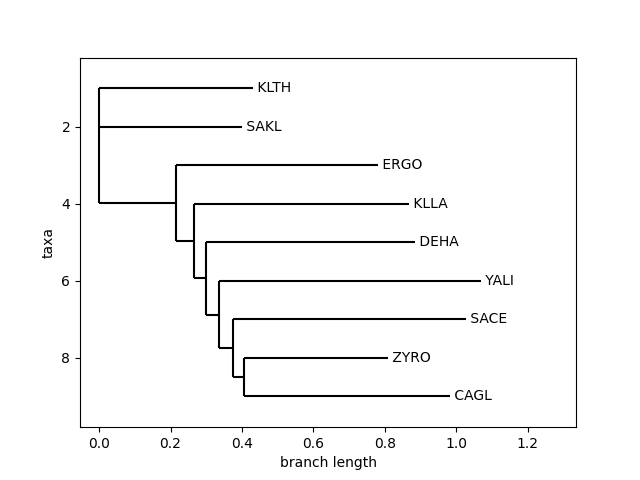
\includegraphics[width=0.7\textwidth]{cons_30}
\end{center}
\end{figure}


\section{Analiza}
Odległość Robinsona-Fouldsa wynosi 6.

Liczba wszystkich krawędzi wynosi 32 (w tym 14 wewnętrznych).

\begin{figure}[H]
\begin{center}
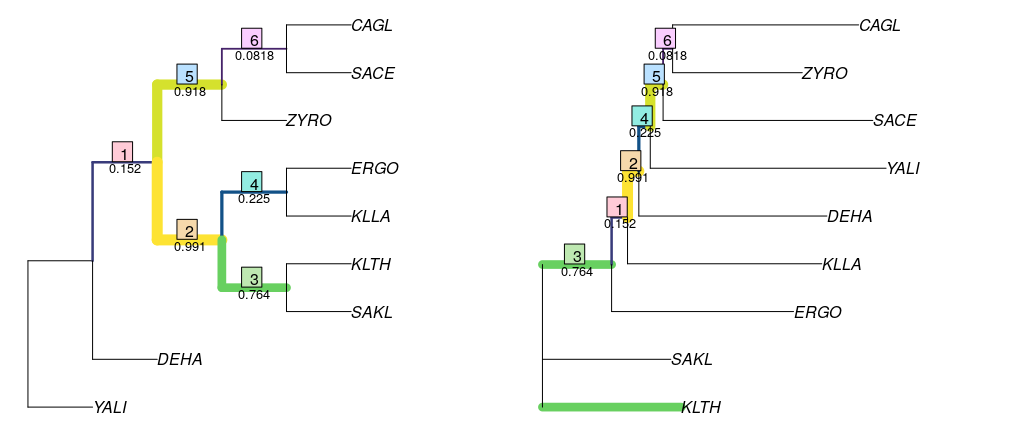
\includegraphics[width=\textwidth]{diff}
\end{center}
\end{figure}

\end{document}

\begin{comment}
BEGIN EXAMPLE PARAGRAPH:

-----Kod w szarym boxie-----
\begin{shaded}\small
\begin{alltt}
KOD
\end{alltt}
\end{shaded}

-----Wstawianie obrazka-----
\begin{figure}[H]
\begin{center}
\includegraphics[width=\textwidth]{raw_url_fasta}
\caption{Przykład umiejscowienia sekwencji przy użyciu surowego linku.}
\end{center}
\end{figure}

-----Tabela-----
\begin{center}
\begin{tabular}{ | l | l | } 
\hline
Nazwa & Dodatek do linku\\ 
\hline
\hline
AC & id\\
\hline
Entry name & entry\%20name\\ 
\hline
Czy Reviewed & reviewed\\ 
\hline
Referencje do Pfam & database(Pfam)\\ 
\hline
Sekwencja & sequence\\ 
\hline
\end{tabular}
\end{center}

\end{comment}